\documentclass[nocover]{pset}
\usepackage{tikz-cd}
\pagestyle{fancy}
\fancyhf{}
\lhead{Forest Kobayashi}
\chead{Algebraic Topology}
\rhead{Math 196 -- Fall, 2018}
\rfoot{\thepage\ of \pageref{LastPage}}
\setlength{\headheight}{15.2pt}
\setlength{\headsep}{10pt}
\lfoot{Friday, October 16th 2018}

\usepackage[normalem]{ulem} % [normalem] prevents the package from
                            % changing the default behavior of `\emph`
                            % to underline.

\titleformat{\section}
  {\LARGE \scshape}{\thesection.}{.5em}{\vspace{.5em}}

\titleformat{\subsection}
  {\Large \scshape}{\thesubsection.}{.5em}{}

\tikzstyle{titlerule}=[dash pattern=on \pgflinewidth off 2pt]
\usetikzlibrary{decorations.markings}

\usepackage{scalerel}
\DeclareMathOperator*{\csum}{\scalerel*{\#}{\sum}}

\newcommand{\wah}[1]{
  \tikz[decoration={markings, mark=between positions 0 and 1 step 3pt
    with { \draw [fill] (0,0) circle [radius=.5pt];}},
  baseline=(todotted.base)]{
  \node[inner sep=0pt,outer sep=0pt] (todotted) {#1};
  \path[postaction={decorate}] (todotted.south west) --
  (todotted.south east);}
}

\newcommand{\udot}[1]{%
    \tikz[baseline=(todotted.base)]{
        \node[inner sep=1pt,outer sep=0pt] (todotted) {#1};
        \draw[titlerule] (todotted.south west) -- (todotted.south east);
    }%
}%
\renewcommand{\epsilon}{\lunateepsilon}
% Homotopy equivalence
\newcommand{\htop}[1][A]{\ensuremath\simeq_{\mrm{rel}\, #1}}
\newcommand{\homm}{\ensuremath\mrm{hom}}
\newcommand{\ob}{\ensuremath\mrm{ob}}
\usepackage{upgreek}

\usetikzlibrary{
  knots,
  hobby,
  decorations.pathreplacing,
  shapes.geometric,
  calc
}

\tikzset{
  knot diagram/every strand/.append style={
    ultra thick,
    blue
  },
  show curve controls/.style={
    postaction=decorate,
    decoration={show path construction,
      curveto code={
        \draw [blue, dashed]
        (\tikzinputsegmentfirst) -- (\tikzinputsegmentsupporta)
        node [at end, draw, solid, blue, inner sep=2pt]{};
        \draw [blue, dashed]
        (\tikzinputsegmentsupportb) -- (\tikzinputsegmentlast)
        node [at start, draw, solid, blue, inner sep=2pt]{}
        node [at end, fill, blue, ellipse, inner sep=2pt]{}
        ;
      }
    }
  },
  show curve endpoints/.style={
    postaction=decorate,
    decoration={show path construction,
      curveto code={
        \node [fill, red, ellipse, inner sep=2pt] at (\tikzinputsegmentlast) {}
        ;
      }
    }
  }
}

\usepackage{caption}

\begin{document}

\begin{center}
  {\scshape \Large Basic Algebraic Topology}

  {\itshape Based on Kosniowski; Matveev}
\end{center}
\vspace{-.1cm}
\hrulefill

\section{Picking up where we left off}
\begin{adjustwidth}{1em}{1em}
  \subsection{Some Theorems}
  We'll breeze briskly through some more point-set topology, then move
  on to the foundations of algebraic topology.
  \begin{theorem}
    Let $Y$ be the quotient space of the topological space $X$
    determined by the surjective mapping $f : X \to Y$. If $X$ is
    compact Hausdorff and $f$ is closed then $Y$ is (compact)
    Hausdorff.
  \end{theorem}
  % \begin{proof}
  %   Let $y_1, y_2 \in Y$, with $y_1 \neq y_2$. Let $X_1 =
  %   f^{-1}(y_1),\ X_2 = f^{-1}(y_2)$. Since $f$ is closed, and every
  %   point of $X$ is closed, then for $X_1, X_2$, take any two
  %   representative elements $x_1$ and $x_2$, and use the fact that
  %   $f(\set{x_1}), f(\set{x_2})$ is the closed image of a close set,
  %   thus $\set{y_1}$ and $\set{y_2}$ are closed in $Y$. Then because
  %   $f$ is continuous, we get $X_1$ and $X_2$ are closed in $X$. Note
  %   too that they must be disjoint, because $y_1 \neq y_2$.
  % \end{proof}
  \begin{corollary}
    Let $X$ be a compact Hausdorff $G$-space with $G$ finite. Then
    $X/G$ is a compact Hausdorff space.
  \end{corollary}
  \begin{corollary}
    If $X$ is a compact Hausdorff space and $A$ is a closed subset of
    $X$ then $X/A$ is a compact Hausdorff space.
  \end{corollary}
  \end{adjustwidth}
  \section{All Together Now\ldots}
  \begin{adjustwidth}{1em}{1em}
  \subsection{Connectedness}~
  \begin{definition}
    Let $(X,\tau)$ a topological space. Then $X$ is said to be
    \emph{connected} iff the only clopen subsets are trivial. If $S
    \subseteq S$, then $S$ is said to be connected iff it is connected
    in the induced topology.

    Equivalently, $X$ is connected iff it cannot be expressed as the
    union of finitely many disjoint non-empty open subsets.
  \end{definition}
  \begin{theorem}
    Let $f : X \to Y$ be continuous, and suppose $X$ is connected.
    Then $Y$ is connected as well.
  \end{theorem}
  \begin{proof}
    Suppose, to obtain a contradiction, that $Y$ is disconnected. Then
    there exist nonempty open sets $U,V \subseteq Y$ with $U \cup V =
    Y$, and $U \cap V = \varnothing$. Since $U,V$ are open and $f$
    continuous, then $f^{-1}(U)$, $f^{-1}(V)$ are open in $X$.
    Furthermore, these are disjoint nonempty subsets of $X$ with
    $f^{-1}(U) \cup f^{-1}(V) = X$. Then $X$ is disconnected, a
    contradiction. Hence $Y$ is connected.
  \end{proof}
  \begin{theorem}
    Suppose that $\set{Y_j \MID j \in J}$ is a collection of connected
    subsets of a space $X$. If $\bigcap_{j \in J} Y_j \neq
    \varnothing$, then $Y = \bigcup_{j \in J} Y_j$ is connected.
  \end{theorem}
  \begin{proof}
    Suppose $U$ is a nonempty clopen subset of $Y$. Then $\exists j
    \in J \st U \cap Y_j \neq \varnothing$. Hence, let $J' = \set{j
      \in J \mid U \cap Y_j \neq \varnothing}$. Then $\forall j' \in
    J'$, we have $U \cap Y_{j'}$ is clopen in the induced topology.
    Since $Y_{j'}$ is connected, it follows that $U \cap Y_{j'} =
    Y_{j'}$. Hence $U = Y$, so $Y$ is connected.
  \end{proof}
  \begin{theorem}
    Let $X,Y$ be topological spaces. Then $X,Y$ are connected iff $X
    \times Y$ is connected.
  \end{theorem}
  \emph{Proof:}
  \begin{iffproof}
  \item Suppose $X,Y$ are connected. $\forall x \in X,\ y \in Y$,
    $X \times \set{y} \cong X$ and $\set{x} \times Y \cong Y$ (and
    thus each is connected), and note $(X \times \set{y}) \cap
    (\set{x} \times Y) \neq \varnothing$, thus by theorem 1.3
    their union is connected. Now, let $y \in Y$ be fixed. Observe
    that
    \[
      X \times Y = \bigcup_{x \in X} (X \times \set{y}) \cap
      (\set{x} \times Y)
    \]
    Hence $X \times Y$ is connected.
  \item Suppose $X \times Y$ is connected. Then since the
    canonical projection maps are continuous, it follows that
    $X,Y$ are connected (continuous image of a connected set is
    connected). \qed
  \end{iffproof}
  \subsection{Path Connectedness}
  We now introduce a new, stronger notion of \emph{connectedness} that
  allows us to treat somewhat pathological examples, such as the
  Topologist's Sine Curve (seen below):
  \begin{figure}[H]
    \centering
    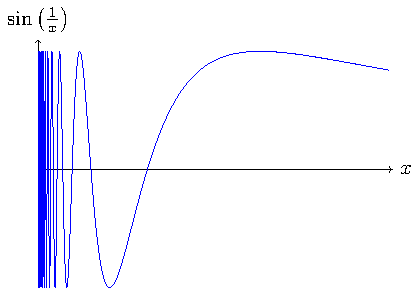
\includegraphics{topsin.pdf}
    \caption{Topolgist's Sine Curve}
  \end{figure}
  Here, if we take the topological space $X = \set{(x,y) \MID y =
    \sin\pn{\frac{1}{x}}} \cup \set{(0,0)}$ under the induced topology
  with respect to $\RR^2$, then we see that $X$ is connected, but
  clearly, there's some\ldots funny business going on near the origin.
  Topologically, there's no problem --- it's impossible to separate
  the origin out from the rest of the points of the curve; no matter
  how close we get, we'll see infinitely many points of the curve
  wobbling around. But clearly, there's no way to actually ``link''
  the origin into the graph. This second point is the idea we want to
  capture with path connectedness. But first, we need to define the
  idea of a path.
  \begin{definition}[Path]
    Let $X$ be a topological space, and let $[0,1] \subseteq \RR$.
    Then if $f : [0,1] \to X$ is a continuous function, we call $f$ a
    \emph{path}. \textbf{Important Note:} $f([0,1])$ is \emph{not} the
    path; rather the mapping $f$ itself is the path. $f([0,1])$ is
    called a \emph{curve}.
  \end{definition}
  In order to apply paths in full, we will first need some handy
  lemmas.
  \begin{lemma}
    Let $f$ be a path in $X$, and let $\ol{f}$ be defined by
    $\ol{f}(t) = f(1-t)$. Then $\ol{f}$ is also a path in $X$.
  \end{lemma}
  \begin{proof}
    Let $g : [0,1] \to [0,1]$ be defined by $g(t) = 1 -t$. Then $g$ is
    continuous. Hence $\ol{f} = f \circ g$ is continuous.
  \end{proof}
  For the next lemma, we actually need another lemma first:
  \begin{lemma}[Gluing Lemma]
    Let $W,X$ be topological spaces and suppose that $W = A \cup B$
    with $A,B$ both closed subsets of $W$. If $f : A \to X$ and $g : B
    \to X$ are continuous functions such that for all $w \in A \cap B$
    $f(w) = g(w)$, then $h : W \to X$ defined by
    \[
      h(w) =
      \begin{cases}
        f(w) & \text{if } w \in A, \\
        g(w) & \text{if } w \in B
      \end{cases}
    \]
    is a continuous function.
  \end{lemma}
  \begin{proof}
    Note that $h$ is well-defined, and let $U$ a closed set in $X$.
    Then
    \begin{align*}
      h^{-1}(U)
      &= \pn{h^{-1}(U) \cap A} \cup \pn{h^{-1}(U) \cap B} \\
      &= f^{-1}(U) \cup g^{-1}(U)
    \end{align*}
    but $f^{-1}(U)$ and $g^{-1}(U)$ are closed, so $h^{-1}(U)$ is
    closed, thus $h$ is a continuous function.
  \end{proof}
  It is worth remarking that an equivalent claim could be proven for
  $A,B$ open.
  \begin{lemma}
    Let $X$ be a topological space, and let $f,g$ be paths in $X$ such
    that $f(1) = g(0)$. Then define the \emph{concatenation} of $f$
    and $g$ (denoted $f * g$) to be the path in $X$ such that
    \[
      f * g (t) =
      \begin{cases}
        f(2t) & \text{if } 0 \leq t \leq \frac{1}{2} \\
        g(2t - 1) & \text{if } \frac{1}{2} \leq t \leq 1
      \end{cases}
    \]
    is a path in $X$.
  \end{lemma}
  \begin{proof}
    Take $A = [0,1/2]$, $B = [1/2, 1]$, and apply the Gluing Lemma.
  \end{proof}
  \begin{definition}[Path connectedness]
    A space $X$ is said to be \emph{path connected} if given any two
    points $x_0, x_1 \in X$, there is a path in $X$ from $x_0$ to
    $x_1$.
  \end{definition}
  Some nice straightforward results follow from the fact that path
  connectedness is defined in terms of continuous functions:
  \begin{theorem}
    Let $X$ be a path-connected topological space, and let $f$ be a
    continuous mapping to a topological space $Y$. Then $f(X)$ is
    path-connected.
  \end{theorem}
  \begin{proof}
    Let $u,v \in Y$. Then $\exists a,b \in X \st f(a) = u,\ f(b) = v$.
    Since $X$ is path connected, there exists a path $g$ in $X$ from
    $a$ to $b$. Then since $f$ is continuous, $f \circ g$ is a path
    from $u$ to $v$ in $Y$.
  \end{proof}
  \begin{theorem}
    Supposet that $\set{Y_i \mid i \in I}$ is a family of path
    connected sets. Then if
    \[
      \bigcap_{i \in I} Y_i \neq \varnothing,
    \]
    then $Y = \bigcup_{i \in I} Y_i$ is path-connected.
  \end{theorem}
  \begin{proof}
    Let $a,b \in Y$, and let $c \in \bigcap_{i \in I} Y_i$. Then
    $\exists i,j \in I \st a \in Y_i, b \in Y_j$. Note that $c \in
    Y_i, Y_j$ as well. Then take a path $f$ in $Y_i$ from $a$ to $c$,
    and a path $g$ in $Y_j$ from $b$ to $c$. Then the path $h = f * g$
    is a path from $a$ to $c$ in $Y$.
  \end{proof}
  \begin{theorem}
    Let $X,Y$ be topological spaces. Then $X$ and $Y$ are path
    connected iff $X \times Y$ is path connected.
  \end{theorem}
  \emph{Proof.}
  \begin{iffproof}
    \item Suppose $X,Y$ are path connected. $\forall x \in X,\ y \in
      Y$, $X \times \set{y} \cong X$ and $\set{x} \times Y \cong Y$
      (and thus each is path connected), and note $(X \times \set{y})
      \cap (\set{x} \times Y) \neq \varnothing$, thus by theorem 2.5
      their union is path connected. Now, let $y \in Y$ be fixed.
      Observe that
      \[
        X \times Y = \bigcup_{x \in X} (X \times \set{y}) \cap
        (\set{x} \times Y)
      \]
      Hence $X \times Y$ is path connected.
    \item Suppose $X \times Y$ is path connected. Then since the
      canonical projection maps are continuous, it follows that $X,Y$
      are path connected (continuous image of a path connected set is
      path connected). \qed
  \end{iffproof}
  \begin{theorem}
    Every path connected space connected. Not every connected space is
    path connected. Oh, also, any non-empty open connected subset of
    $\RR$ is path connected.
  \end{theorem}

  \section{A Brief Discussion of Manifolds}

  \begin{definition}[Manifolds]
    Let $n \in \ZZ^{>0}$, and let $(M, \tau)$ be a topological space.
    Then $M$ is called a manifold iff $M$ is Hausdorff, and $\forall m
    \in M$, there exists a neighborhood $N$ of $m$ such that $N \cong
    \mathring{D}^n = \set{x \in \RR^n \MID \norm{x} < 1}$.
  \end{definition}
  \begin{definition}[Connected Sum]
    Let $S_1$, $S_2$ be compact connected 2-manifolds (surfaces), and
    let $D_1 \subseteq S_1$, $D_2 \subseteq S_2$ with $D_1, D_2 \cong
    D^2$. Let $h_1 : D_1 \to D^2$, and $h_2 : D_2 \to D^2$ be
    homeomorphisms. Then define $\sim$ to be an equivalence relation
    such that $x \sim h^{-1}_2 h_1(x)$ iff $x \in \partial D_1$, and
    $x \sim x$ otherwise. Then $S_1 \# S_2$ is given by
    \[
      \frac{(S_1 - \mathring{D_1}) \cup (S_2 - \mathring{D_2})}{\sim}
    \]
  \end{definition}
  \begin{definition}
    Call a surface $S^2$ \emph{orientable} if it contains no
    M\"{o}bius strip, and \emph{non-orientable} otherwise. Then for $m
    \geq 0, n \geq 1$, we call
    \[
      S^2 \# \pn{\csum_{i=1}^m T} = S \# mT
    \]
    the \emph{standard orientable surface of genus $m$}, and
    \[
      S^2 \# \pn{\csum_{i=1}^n \RR P^2} = S \# n\RR P^2
    \]
    the \emph{standard non-orientable surface of genus $n$}.
  \end{definition}

\end{adjustwidth}
\section{Homotopy}
\begin{adjustwidth}{1em}{1em}
  We are now ready to introduce a concept that will be of fundamental
  importance later on. In a nutshell, this is the idea of
  \emph{equivalent maps}, as motivated by the following
  uncharacteristically-unprofessional diagram:
  \begin{figure}[H]
    \centering
    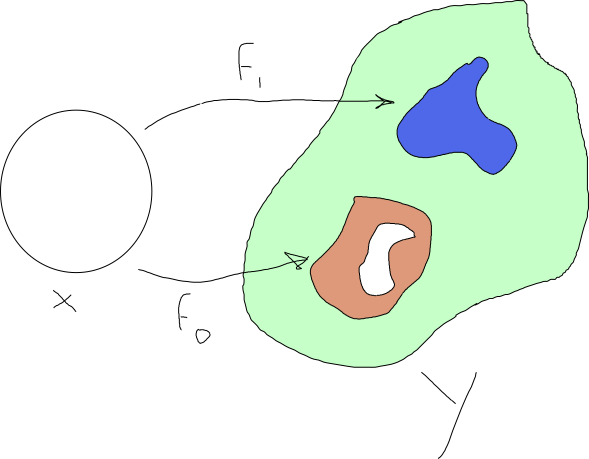
\includegraphics[width=5cm,keepaspectratio=true]{sad_diagram.png}
    \caption{I'm not as good with inkscape as Prof.\ Nelson is}
  \end{figure}
  $f_0$ and $f_1$ are, in some sense, fundamentally not the same as
  each other, as one contains a hole while the other does not. To make
  this precise, we define the idea of homotopy equivalence:
  \begin{definition}
    Let $X,Y$ be topological spaces, and let $f_0, f_1 : X \to Y$.
    Then say $f_0, f_1$ are \emph{homotopic} iff there is a continuous
    map $F : X \times I \to Y$ such that $F(x,0) = f_0(x)$ and $F(x,1)
    = f_1(x)$. In this case we write $f_0 \simeq f_1$, and call the
    map $F$ a \emph{homotopy} between $f_0$ and $f_1$. For each $t \in
    [0,1]$, we denote $F(x,t)$ by $f_t(x)$.
  \end{definition}
  Some part of me really just wants to draw a commutative diagram
  here, but it doesn't quite feel appropriate. Anyways, note that a
  homotopy essentially amounts to a path through the space of
  continuous maps between topological spaces. Also, observe that our
  definition might not yet be perfectly desirable, as it allows us to
  make paths homotopic to points. Hence, we define the notion of a
  \emph{relative homotopy}.
  \begin{definition}
    Let $X$ be a topological space, and let $A \subseteq X$. Suppose
    that $f_0, f_1 : X \to Y$ are continuous. Then we say $f_0$ and
    $f_1$ are \emph{homotopic relative to $A$} iff there exists a
    homotopy $F : X \times I \to Y$ between $f_0$ and $f_1$ such that
    $F(a,t)$ does not depend on $t$ for any $a \in A$. That is,
    $\forall a \in A, t \in I$, $F(a,t) = f_0(a)$. In this case, we
    say $F$ is a \emph{homotopy relative to $A$}, and we write $f_0
    \simeq f_1 (\mrm{rel} A)$, or $f_0 \simeq_{\mrm{rel} A} f_1$.
  \end{definition}
  Less rigorously, this essentially amounts to the homotopy
  \emph{leaving $A$ alone}. Note that if $A = \set{0,1}$, homotopy
  relative to $A$ means that we can't always get some map ``over an
  obstacle.''
  \begin{lemma}
    $\htop$ is an equivalence relation on $\homm(X,Y)$.
  \end{lemma}
  \begin{proof}
    First, observe that $\htop$ is reflexive: take $F(x,t) = f_0(x)$.
    Symmetry follows from the fact that if $F(x,t)$ is a homotopy,
    then $F(x, 1-t)$ is a homotopy. Finally, note that if we have $f
    \htop g$ and $g \htop h$, then we can simply concatenate the
    homotopys from $f$ to $g$ and $g$ to $h$ to yield one from $f$ to
    $h$.
  \end{proof}
  We can now apply this new shiny tool to some classifications of
  topological spaces.
  \begin{definition}
    Let $X$, $Y$ be topological spaces. We say $X$ and $Y$ are
    \emph{of the same homotopy type} if there exist continuous maps $f
    : X \to Y$, $g : Y \to X$ such that $gf \simeq 1 : X \to X$, $fg
    \simeq 1 : Y \to Y$.
  \end{definition}
  Ok, there \emph{really} feels like there's some category nonsense
  going on here. Anyways, note that we did \emph{not} use relative
  homotopy here. That was 100\% intentional --- in a sense, we want
  homotopy equivalence to encode information about retraction and
  stretching that can be lossy in ways that homeomorphism cannot.
  Homeomorphism is rigid about exact equivalence, homotopy equivalence
  lets us fudge things a little bit. For instance, a m\"{o}bius band
  is certainly not homeomorphic to a cylinder, whereas the two are
  both homotopy equivalent to a circle.
  \begin{definition}
    A space $X$ is said to be \emph{contractible} if it is homotopy
    equivalent to a point.
  \end{definition}
  \begin{definition}
    A subset $A$ of a topological space $X$ is called a \emph{retract}
    of $X$ iff there is a continuous map $r : X \to A$ such that
    $r\imath = 1 : A \to A$, where $\imath$ is the inclusion map.
    Equivalently, $r | A = 1$. Under these conditions, $r$ is called
    an \emph{inclusion} map.
  \end{definition}
  %% Wait this is false I think. I think this might actually be true
  %% for a deformation retract, though?
  % Note that here, the continuity condition on $r$ essentially requires
  % that we be shrinking our space in until it rests on the boundary.
  \begin{definition}
    A subset $A \subseteq X$ is called a \emph{deformation retract} of
    $X$ if there is a retraction $r : X \to A$ such that $\imath r
    \simeq 1 : X \to X$.
  \end{definition}
  If $A$ is a deformation retract of $X$, it follows that $A$ and $X$
  are homotopy equivalent.
  \begin{definition}
    Let $X$ be a topological space, and $A \subseteq X$. Then call $A$
    a \emph{strong deformation retract} iff there is a retraction $r :
    X \to A$ such that $\imath r \htop 1 : X \to X$.
  \end{definition}
  Essentially, a strong deformation retract is a way of deforming $X$
  within itself to $A$, while keeping $A$ fixed.
  % Essentailly, we require that, upon performing our retraction, things
  % end up more or less ``where they should be,'' and don't jump to a
  % point in $A$ discontinuously.
\end{adjustwidth}
\section{Towards the fundamental group}
\begin{adjustwidth}{1em}{1em}
  \subsection{Group Structure of Paths}
  Recall that we defined the concatenation of two paths $f$ and $g$ to
  be $f * g$, provided $f(1) = g(0)$. In preparation for a discussion
  of the fundamental group, we wish to investigate this further. In
  particular, we'll be interested in looking at the extent to which
  equivalence classes of paths (under homotopy relative to a
  particular choice of $A$) exhibit the structure of a group. This,
  ultimately, will be what allows us to escape the sadness of
  point-set topology, and transition to some truly beautiful
  mathematics.
  \begin{definition}
    Let $X$ be a topological space, and let $f,g$ be paths in $X$. We
    say $f$ and $g$ are \emph{equivalent} iff $f$ and $g$ are
    homotopic relative to $\set{0,1}$, in which case we write $f \sim
    g$. The equivalence classes of $f$ are denoted by $[f]$.
  \end{definition}
  Note that if $f$ and $g$ are equivalent, then the homotopy is some
  continuous function $F: I \times I \to X$ such that
  \begin{align*}
    F(t,0) = f_0(t) \quad \text{and} &\quad F(t, 1) = f_1(t) \,\,\quad t
    \in I\\
    F(0,s) = f_0(0) \quad \text{and} &\quad F(1, s) = f_0(1) \quad s
    \in I
  \end{align*}
  Hence, in a bit of an abuse of notation, we write $F : f_0 \sim
  f_1$.
  \begin{theorem}
    Let $X$ be a topological space, and let $f,g,h$ be paths in $X$.
    Then
    \begin{enumerate}[label=\arabic*)]
      \item $[f][g] = [f*g]$
      \item $[f]([g][h]) = ([f][g])[h]$ (whenever the product is
        defined --- note though that in general, $(f * g) * h \neq f *
        (g * h)$. But, we have the next-best thing: if $f(1) = g(0)$
        and $g(1) = h(0)$, then $(f * g) * h \sim f * (g * h)$).
      \item If $x \in X$, then define $\epsilon_x : I \to X$ by
        $\epsilon_x(t) = x$. Then $[\epsilon_x][f] = [f] =
        [f][\epsilon_y]$ if $f$ begins at $x$ and ends at $y$.
      \item Let $x = f(0)$, and $y = f(1)$. Then $[f][\ol{f}] =
        [\epsilon_x]$, and $[\ol{f}][f] = [\epsilon_y]$.
    \end{enumerate}
  \end{theorem}
  Hence, we see that the equivalence classes of paths on $X$
  \emph{almost} behave like a group. If only multiplication were
  always defined, and we had $x=y$\ldots
  \subsection{The Fundamental Group}
  The trick is to make it happen.
  \begin{definition}
    Let $X$ be a topological space, and let $f$ be a path in $X$. Then
    $f$ is said to be \emph{closed} if $f(0) = f(1)$. If $f(0) = f(1)
    = x$, then we say $f$ is \emph{based} at $x$.
  \end{definition}
  Oh look. We made it happen. How, you might ask? Well, observe:
  \begin{definition}[Fundamental Group]
    Let $X$ be a topological space, and let $x \in X$. Let $f$ be some
    closed path based at $x$. Then define the \emph{fundamental group}
    of $X$ with base point $x$ (denoted $\pi(X,X)$) to be $[f]$.
  \end{definition}
  That this is a group follows immediately from Theorem 5.1. Buckle
  your seatbelts everyone, things are about to get \emph{really}
  snazzy.
  \begin{theorem}
    Let $x,y \in X$. If there is a path in $X$ from $x$ to $y$, then
    $\pi(X,x)$ and $\pi(X,y)$ are isomorphic.
  \end{theorem}
  \begin{proof}
    Let $f$ be a path in $X$ from $x$ to $y$. Then for all $g \in
    \pi(X,x)$, $[\ol{f}] * [g] * [f] = [\ol{f} * g * f]$ is an
    equivalence class of paths in $\pi(X,y)$. Hence, define $\varphi :
    \pi(X,x) \to \pi(X,y)$ by
    \[
      \varphi_{f}([g]) = [\ol{f} * g * f].
    \]
    Clearly, this is bijective (we can define $\varphi_{f}^{-1}(h) =
    [f * h * \ol{f}]$, and note that $\varphi_f^{-1} \varphi =
    1_{\pi(X,x)}$, $\varphi_f \varphi_f^{-1} = 1_Y$), and inherits the
    group structure of $\pi(X,x)$ in its image (since it is a
    conjugation). Thus it is a homomorphism.
  \end{proof}
  \begin{corollary}
    Let $X$ be a path connected topological space. Then for all $x,y
    \in X$, $\pi(X,x) \cong \pi(X,y)$.
  \end{corollary}
  Note that the requirement that $X$ be \emph{path} connected is
  essential.
  \subsection{Continuous Functions \& Fundamental Groups}
  We want to understand how continuous functions affect the
  fundamental group. First, we have the following three facts:
  \begin{lemma}
    Let $X$, $Y$ be topological spaces, and let $\varphi : X \to Y$ be
    continuous. Then
    \begin{enumerate}[label=\arabic*)]
      \item If $f,g$ are paths in $X$, then $\varphi f$, $\varphi g$
        are paths in $Y$.
      \item If $f \sim g$, then $\varphi f \sim \varphi g$
      \item If $f$ is a closed path in $X$ based at $x \in X$, then
        $\varphi f$ is a closed path in $Y$ based at $\varphi(x)$
    \end{enumerate}
  \end{lemma}
  From these facts, we might deduce that continuous maps are, on some
  level, really just performing a sort of group homomorphism.
  \begin{definition}[Induced Homomorphism]
    Let $X, Y$ be topological spaces, and let $\varphi : X \to Y$ be
    continuous. Then define the \emph{induced homomorphism} as
    follows: for all $x \in X$, define $\varphi_* : \pi(X,x) = \pi(Y,
    \varphi(x))$ such that if $f$ is a path based on $x$,
    \[
      \varphi_*([f]) = [\varphi f].
    \]
  \end{definition}
  We referred to this as a homomorphism, so it better actually be one.
  Let's prove it!
  \begin{theorem}
    Let $X,Y$ be topological spaces, and let $\varphi : X \to Y$ be
    continuous. Then $\varphi_*$ is a homomorphism of groups.
  \end{theorem}
  \begin{proof}
    Let $[f], [g] \in \pi(X,x)$. Then
    \begin{align*}
      \varphi_*\pn{[f]*[g]}
      &= \varphi_*([f * g]) \\
      &= [\varphi(f * g)] \\
      &= [\varphi(f) * \varphi(g)] \tag{*}\\
      &= [\varphi(f)] * [\varphi(g)]
    \end{align*}
    note that $(*)$ follows by simply cutting any representative path
    halfway through, and doing the work. Hence, $\varphi_*$ is a group
    homomorphism.
  \end{proof}
  A number of nice properties follow.
  \begin{theorem}
    Let $X,Y,Z$ be topological spaces, and let $\varphi : X \to Y$,
    $\psi : Y \to Z$ be continuous maps. Then
    \begin{enumerate}[label=\arabic*)]
      \item $(\psi \varphi)_* = \psi_* \varphi_*$
      \item If $1 : X \to X$ is the identity map then $1_*$ is the
        identity homomorphism.
      \item If $\varphi$ is a homeomorphism, then $\varphi_* :
        \pi(X,x) \to \pi(Y, \varphi(x))$ is an isomorphism of groups.
    \end{enumerate}
  \end{theorem}
  Instead of proving these, we make a remark about functors. Recall
  the following definition:
  \begin{definition}[Functor]
    Let $\mb C, \mb D$ be categories, and let $c \in \ob(C)$, $f,g \in
    \homm(C)$. Then call $\mc{F} = (\mc{F}_o, \mc{F}_a)$ a functor if
    \[
      \mc{F}_o : \ob(\mb C) \to \ob(\mb D) \qquad \mc{F}_a : \homm(\mb
      C) \to \homm(\mb D)
    \]
    such that the following essential properties are preserved:
    \begin{enumerate}
    \item $\forall (f : c \to c') \in \homm(\mb C)$, $\mc{F}_a(f) :
      \mc{F}_o(c) \to \mc{F}_o(c')$, with
      \[
        \mc{F}_a(1_{c}) = 1_{\mc{F}_o(c)}
      \]
      and
    \item
      \[
        \mc{F}_a(g \circ f) = \mc{F}_a(g) \circ \mc{F}_a(f).
      \]
    \end{enumerate}
  \end{definition}
  Or alternatively, with homsets:
  \begin{definition}[Functor (version 2)]
    Let $\mc{T} : \mb{C} \to \mb{B}$ be defined with the usual object
    functor $\mc{T}_o$, together with a collection of functions
    \[
      \mc{T}^{a,b} : \homm_{\mb C}(a,b) \to \homm_{\mb B}(\mc{T}_o(a),
      \mc{T}_o(b))
    \]
    then $\mc{T}$ is \emph{full} when every such $\mc{T}^{a,b}$ is
    surjective, and \emph{faithful} when injective.
  \end{definition}
  We can now frame the results obtained above in the language of
  category theory.
  \begin{theorem}
    Let $\mb{Top}_*$ denote the category with objects $(X,x)$ where
    $X$ is a topological space, and $x$ is a selected base point.
    Define the morphisms on $\mb{Top}_*$ to be continuous maps of the
    form $\varphi : (X, x) \to (Y, y)$, where we require $\varphi(x) =
    y$. Then the map $\mc F : \mb{Top}_* \to \mb{Grp}$ taking each
    $(X,x)$ to the corresponding fundamental group is a functor.
  \end{theorem}
  \begin{proof}
    Take
    \[
      \mc F_o((X,x)) = \pi(X,x) \qquad \qquad \mc F_a(\varphi) =
      \varphi_*.
    \]
    And note that indeed, as we defined above, if $\varphi : (X,x) \to
    (Y,y)$, then $\varphi_* : \pi(X,x) \to \pi(Y,y)$, and $\mc
    F_a(1_{(X,x)}) = 1_*$, and indeed $\mc F_a(\psi \circ \varphi) =
    \mc F_a(\psi) \circ \mc F_a(\varphi)$. Hence $\mc F$ is a functor.
  \end{proof}
\end{adjustwidth}
\end{document}
